\clearpage

\section{Transparent with 1+1 Protection}
In this case study we focus on the transparent case with 1 + 1 protection.
In this mode of transport, the information travels in a route defined through optical channels between origin and destination nodes always in the optical domain and, consequently, physical topology and logical topology are different.
An advantage of this mode of transport is the possibility of transporting express traffic.
An disadvantage is that the capacity utilization of the optical channels is worse than in the opaque mode of transport due to grooming only customer signs with the same endpoints.

\subsection{Physical Network Topology}
\begin{tcolorbox}	
\begin{tabular}{p{2.75cm} p{0.2cm} p{10.5cm}} 	
\textbf{Student Name}  &:& Tiago Esteves    (October 03, 2017 - )\\
\textbf{Goal}          &:& Implement the dimensioning of optical networks in the transparent transport mode.
\end{tabular}
\end{tcolorbox}
\vspace{-5pt}

\subsubsection{Reference Network}
In the figure below we ca see that our reference network consists of 6 nodes and 8 Bidirectional links.
The matrix of distances between the respective nodes and the ODU's matrices are the same as those reported in the opaque transport mode.

\begin{figure}[h!]
\centering
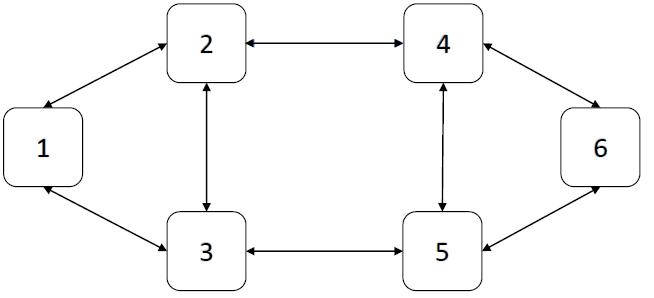
\includegraphics[width=\textwidth]{RedeTeste}
\caption{Physical Topology of the Reference Network.}
\end{figure}

The distance matrix is the same for the two scenarios but the ODU's matrices are not.
In this case only the matrices for the case of high traffic are elucidated, being that in the case of a low traffic it is only necessary to divide these matrices by the value 10.

\[
Dist=
  \begin{bmatrix}
    0 & 500 & 500 & 0 & 0 & 0 \\
    500 & 0 & 400 & 500 & 0 & 0 \\
    500 & 400 & 0 & 0 & 500 & 0 \\
    0 & 500 & 0 & 0 & 600 & 450 \\
    0 & 0 & 500 & 600 & 0 & 550 \\
    0 & 0 & 0 & 450 & 550 & 0
  \end{bmatrix}
\quad ODU0=
  \begin{bmatrix}
    0 & 50 & 10 & 30 & 10 & 30 \\
    50 & 0 & 0 & 10 & 50 & 0 \\
    10 & 0 & 0 & 10 & 40 & 10 \\
    30 & 10 & 10 & 0 & 10 & 0 \\
    10 & 50 & 40 & 10 & 0 & 30 \\
    30 & 0 & 10 & 10 & 30 & 0
  \end{bmatrix}
\]
\[
ODU1=
  \begin{bmatrix}
    0 & 20 & 40 & 20 & 0 & 50 \\
    20 & 0 & 0 & 30 & 10 & 10 \\
    40 & 0 & 0 & 10 & 10 & 0 \\
    30 & 30 & 10 & 0 & 10 & 30 \\
    0 & 10 & 10 & 10 & 0 & 10 \\
    50 & 10 & 0 & 30 & 10 & 0
  \end{bmatrix}
\quad ODU2=
  \begin{bmatrix}
    0 & 10 & 10 & 10 & 0 & 0 \\
    10 & 0 & 0 & 0 & 10 & 0 \\
    10 & 0 & 0 & 10 & 10 & 0 \\
    10 & 0 & 10 & 0 & 10 & 0 \\
    0 & 10 & 10 & 10 & 0 & 10 \\
    0 & 0 & 0 & 0 & 10 & 0
  \end{bmatrix}
\]
\[
ODU3=
  \begin{bmatrix}
    0 & 0 & 0 & 0 & 0 & 0 \\
    0 & 0 & 10 & 0 & 0 & 10 \\
    0 & 10 & 0 & 0 & 10 & 0 \\
    0 & 0 & 0 & 0 & 0 & 0 \\
    0 & 0 & 10 & 0 & 0 & 0 \\
    0 & 10 & 0 & 0 & 0 & 0
  \end{bmatrix}
\qquad ODU4=
  \begin{bmatrix}
    0 & 0 & 0 & 0 & 0 & 0 \\
    0 & 0 & 0 & 0 & 0 & 10 \\
    0 & 0 & 0 & 0 & 0 & 0 \\
    0 & 0 & 0 & 0 & 0 & 0 \\
    0 & 0 & 0 & 0 & 0 & 10 \\
    0 & 10 & 0 & 0 & 10 & 0
  \end{bmatrix}
\]

\vspace{17pt}

The values indicated in the distance matrix, referred to below, are expressed in kilometers (Km) and as it couldn't be otherwise, this matrix is symmetric.
In relation to the traffic matrices each ODU, referred previously, has its respective value being that the ODU0 corresponds to 1.25 Gbits/s, ODU1 to 2.5 Gbits/s, ODU2 to 10 Gbits/s, ODU3 to 40 Gbits/s and finally the ODU4 corresponds to 100 Gbits/s.
As we can see these matrices are bidirectional because they are symmetric matrices and as such the traffic sent in one direction must be the same traffic sent in the opposite direction. \\

Through these ODU's we can calculate total network traffic for the low traffic scenario:\\

$T_1^0$ = 600x1.25 = 750 Gbits/s \quad
$T_1^1$ = 500x2.5 = 1250 Gbits/s \quad
$T_1^2$ = 160x10 = 1600 Gbits/s \\

$T_1^3$ = 60x40 = 2400 Gbits/s \quad
$T_1^4$ = 40x100 = 4000 Gbits/s \\

$T_{1total}$ = 750 + 1250 + 1600 + 2400 + 4000 = 10000 Gbits/s \qquad
$T_{total}$ = 10000/2 = 5 Tbits/s\\

Where the variable $T_1^x$ represents the unidirectional traffic of the ODUx, for example, $T_1^0$ represents the unidirectional traffic of the ODU0 and $T_1^1$ represents the unidirectional traffic of the ODU1. The variable $T_{1}$ represents the total of unidirectional traffic that is injected into the network and finally the variable $T$ represents the total of bidirectional traffic.\\

We can thus conclude that the total traffic for the two scenarios is as follows:
\begin{itemize}
  \item Low Traffic: \textbf{0.5 TBits/s}
  \item High Traffic: \textbf{5 TBits/s}
\end{itemize}

Finally for this project has to take into consideration the table \ref{table:3} because in it we can see the values of the variables associated with this network.
\begin{table}[h!]
\centering
\begin{tabular}{|| c | c | c||}
 \hline
 Constant & Description & Value \\
 \hline\hline
 N & Number of nodes & 6 \\
 L & Number of bidirectional links & 8 \\
 <$\delta$> & Node out-degree & 2.667 \\
 <len> & Mean link length (km) & 500 \\
 <h> & Mean number of hops for working paths & 1.533 \\
 <h'> & Mean number of hops for backup paths & 2.467 \\
 \hline
\end{tabular}
\caption{Table of reference network values}
\label{table:3}
\end{table}


\subsubsection{Realistic Network}
The real network chosen for this work is the EON (European Optical Network).

\begin{figure}[h!]
\centering
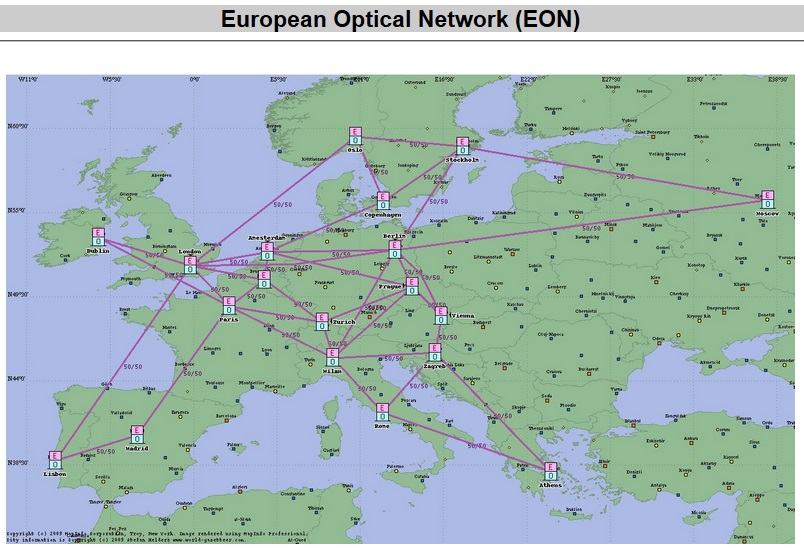
\includegraphics[width=\textwidth]{EON_Rede_Realista}
\caption{Physical Topology of the Realistic Network.}
\end{figure}

Through the previous figure we can see how nodes are organized geographically and the distance matrix created on the next page is constructed based on real distances between them.
For a better understanding of the distances matrix the table \ref{city_nodes_t} was created to assign to each city a number of a node in the network.

\begin{table}[h!]
\centering
\begin{tabular}{|| c | c ||}
 \hline
 City & Node \\
 \hline\hline
 Oslo & 1 \\
 Stockholm & 2 \\
 Moscow & 3 \\
 Copenhagen & 4 \\
 Berlin & 5 \\
 Prague & 6 \\
 Vienna & 7 \\
 Zagreb & 8 \\
 Athens & 9 \\
 Rome & 10 \\
 Milan & 11 \\
 Zurich & 12 \\
 Brussels & 13 \\
 Amesterdan & 14 \\
 London & 15 \\
 Dublin & 16 \\
 Paris & 17 \\
 Madrid & 18 \\
 Lisbon & 19 \\
 \hline
\end{tabular}
\caption{Table of city and respective node}
\label{city_nodes_t}
\end{table}

In this real case we have once again to take into consideration the table \ref{table:4} because it is through it that we can see the values of the variables associated with this network.

\begin{table}[h!]
\centering
\begin{tabular}{|| c | c | c||}
 \hline
 Constant & Description & Value \\
 \hline\hline
 N & Number of nodes & 19 \\
 L & Number of bidirectional links & 37 \\
 <$\delta$> & Node out-degree & 3.89 \\
 <len> & Mean link length (km) & 753.76 \\
 <h> & Mean number of hops for working paths & 2.3 \\
 <h'> & Mean number of hops for backup paths & 3.2 \\
 \hline
\end{tabular}
\caption{Table of realistic network values}
\label{table:4}
\end{table}

The values indicated in the distance matrix, referred to below, are expressed in kilometers (Km).
For this network we must also create matrices of ODU's to determine the total traffic used in each scenario  but in this case only the matrices for high traffic are elucidated.


\begin{sidewaysfigure}

\[
Dist=
  \begin{pmatrix}
    0 & 417 & 0 & 484 & 0 & 0 & 0 & 0 & 0 & 0 & 0 & 0 & 0 & 0 & 1155 & 0 & 0 & 0 & 0 \\
    417 & 0 & 1228 & 523 & 811 & 0 & 0 & 0 & 0 & 0 & 0 & 0 & 0 & 0 & 0 & 0 & 0 & 0 & 0 \\
    0 & 1228 & 0 & 0 & 1611 & 0 & 0 & 0 & 0 & 0 & 0 & 0 & 0 & 0 & 0 & 0 & 0 & 0 & 0 \\
    484 & 523 & 0 & 0 & 0 & 0 & 0 & 0 & 0 & 0 & 0 & 0 & 0 & 622 & 0 & 0 & 0 & 0 & 0 \\
    0 & 811 & 1611 & 0 & 0 & 281 & 524 & 0 & 0 & 0 & 843 & 0 & 0 & 577 & 933 & 0 & 0 & 0 & 0 \\
    0 & 0 & 0 & 0 & 281 & 0 & 251 & 0 & 0 & 0 & 646 & 527 & 0 & 712 & 0 & 0 & 0 & 0 & 0 \\
    0 & 0 & 0 & 0 & 524 & 251 & 0 & 268 & 0 & 0 & 0 & 0 & 0 & 0 & 0 & 0 & 0 & 0 & 0 \\
    0 & 0 & 0 & 0 & 0 & 0 & 268 & 0 & 1081 & 518 & 530 & 0 & 0 & 0 & 0 & 0 & 0 & 0 & 0 \\
    0 & 0 & 0 & 0 & 0 & 0 & 0 & 1081 & 0 & 1052 & 0 & 0 & 0 & 0 & 0 & 0 & 0 & 0 & 0 \\
    0 & 0 & 0 & 0 & 0 & 0 & 0 & 518 & 1052 & 0 & 477 & 0 & 0 & 0 & 0 & 0 & 0 & 0 & 0 \\
    0 & 0 & 0 & 0 & 843 & 646 & 0 & 530 & 0 & 477 & 0 & 219 & 0 & 0 & 0 & 0 & 640 & 0 & 0 \\
    0 & 0 & 0 & 0 & 0 & 646 & 0 & 0 & 0 & 0 & 219 & 0 & 493 & 0 & 0 & 0 & 488 & 0 & 0 \\
    0 & 0 & 0 & 0 & 0 & 0 & 0 & 0 & 0 & 0 & 0 & 493 & 0 & 173 & 321 & 0 & 264 & 0 & 0 \\
    0 & 0 & 0 & 622 & 577 & 712 & 0 & 0 & 0 & 0 & 0 & 0 & 173 & 0 & 358 & 0 & 0 & 0 & 0 \\
    1155 & 0 & 0 & 0 & 933 & 0 & 0 & 0 & 0 & 0 & 0 & 0 & 321 & 358 & 0 & 464 & 344 & 0 & 1587 \\
    0 & 0 & 0 & 0 & 0 & 0 & 0 & 0 & 0 & 0 & 0 & 0 & 0 & 0 & 464 & 0 & 782 & 0 & 0 \\
    0 & 0 & 0 & 0 & 0 & 0 & 0 & 0 & 0 & 0 & 640 & 488 & 264 & 0 & 344 & 782 & 0 & 1054 & 0 \\
    0 & 0 & 0 & 0 & 0 & 0 & 0 & 0 & 0 & 0 & 0 & 0 & 0 & 0 & 0 & 0 & 1054 & 0 & 503 \\
    0 & 0 & 0 & 0 & 0 & 0 & 0 & 0 & 0 & 0 & 0 & 0 & 0 & 0 & 1587 & 0 & 0 & 503 & 0
  \end{pmatrix}
\]
\end{sidewaysfigure}

\[
ODU0=
  \begin{bmatrix}
    0 & 10 & 10 & 10 & 10 & 10 & 10 & 10 & 10 & 10 & 10 & 10 & 10 & 10 & 10 & 10 & 10 & 10 & 10 \\
    10 & 0 & 10 & 10 & 10 & 10 & 10 & 10 & 10 & 10 & 10 & 10 & 10 & 10 & 10 & 10 & 10 & 10 & 10 \\
    10 & 10 & 0 & 10 & 10 & 10 & 10 & 10 & 10 & 10 & 10 & 10 & 10 & 10 & 10 & 10 & 10 & 10 & 10 \\
    10 & 10 & 10 & 0 & 10 & 10 & 10 & 10 & 10 & 10 & 10 & 10 & 10 & 10 & 10 & 10 & 10 & 10 & 10 \\
    10 & 10 & 10 & 10 & 0 & 10 & 10 & 10 & 10 & 10 & 10 & 10 & 10 & 10 & 10 & 10 & 10 & 10 & 10 \\
    10 & 10 & 10 & 10 & 10 & 0 & 10 & 10 & 10 & 10 & 10 & 10 & 10 & 10 & 10 & 10 & 10 & 10 & 10 \\
    10 & 10 & 10 & 10 & 10 & 10 & 0 & 10 & 10 & 10 & 10 & 10 & 10 & 10 & 10 & 10 & 10 & 10 & 10 \\
    10 & 10 & 10 & 10 & 10 & 10 & 10 & 0 & 10 & 10 & 10 & 10 & 10 & 10 & 10 & 10 & 10 & 10 & 10 \\
    10 & 10 & 10 & 10 & 10 & 10 & 10 & 10 & 0 & 10 & 10 & 10 & 10 & 0 & 0 & 0 & 0 & 0 & 0 \\
    10 & 10 & 10 & 10 & 10 & 10 & 10 & 10 & 10 & 0 & 0 & 0 & 0 & 0 & 0 & 0 & 0 & 0 & 0 \\
    10 & 10 & 10 & 10 & 10 & 10 & 10 & 10 & 10 & 0 & 0 & 0 & 0 & 0 & 0 & 0 & 0 & 0 & 0 \\
    10 & 10 & 10 & 10 & 10 & 10 & 10 & 10 & 10 & 0 & 0 & 0 & 0 & 0 & 0 & 0 & 0 & 0 & 0 \\
    10 & 10 & 10 & 10 & 10 & 10 & 10 & 10 & 10 & 0 & 0 & 0 & 0 & 0 & 0 & 0 & 0 & 0 & 0 \\
    10 & 10 & 10 & 10 & 10 & 10 & 10 & 10 & 0 & 0 & 0 & 0 & 0 & 0 & 0 & 0 & 0 & 0 & 0 \\
    10 & 10 & 10 & 10 & 10 & 10 & 10 & 10 & 0 & 0 & 0 & 0 & 0 & 0 & 0 & 0 & 0 & 0 & 0 \\
    10 & 10 & 10 & 10 & 10 & 10 & 10 & 10 & 0 & 0 & 0 & 0 & 0 & 0 & 0 & 0 & 0 & 0 & 0 \\
    10 & 10 & 10 & 10 & 10 & 10 & 10 & 10 & 0 & 0 & 0 & 0 & 0 & 0 & 0 & 0 & 0 & 0 & 0 \\
    10 & 10 & 10 & 10 & 10 & 10 & 10 & 10 & 0 & 0 & 0 & 0 & 0 & 0 & 0 & 0 & 0 & 0 & 0 \\
    10 & 10 & 10 & 10 & 10 & 10 & 10 & 10 & 0 & 0 & 0 & 0 & 0 & 0 & 0 & 0 & 0 & 0 & 0
  \end{bmatrix}
\]

\vspace{15pt}

\[
ODU1=
  \begin{bmatrix}
    0 & 10 & 0 & 0 & 0 & 0 & 0 & 0 & 0 & 0 & 10 & 10 & 10 & 10 & 10 & 10 & 10 & 0 & 0 \\
    10 & 0 & 0 & 0 & 0 & 0 & 0 & 0 & 0 & 0 & 10 & 10 & 10 & 10 & 10 & 10 & 10 & 10 & 10 \\
    0 & 0 & 0 & 0 & 0 & 10 & 10 & 10 & 10 & 10 & 10 & 10 & 10 & 10 & 10 & 10 & 10 & 10 & 10 \\
    0 & 0 & 0 & 0 & 10 & 10 & 10 & 10 & 10 & 10 & 10 & 10 & 10 & 10 & 10 & 10 & 10 & 10 & 10 \\
    0 & 0 & 0 & 10 & 0 & 10 & 10 & 10 & 10 & 10 & 10 & 10 & 10 & 10 & 10 & 10 & 10 & 10 & 10 \\
    0 & 0 & 10 & 10 & 10 & 0 & 10 & 10 & 10 & 10 & 10 & 10 & 10 & 10 & 10 & 10 & 10 & 10 & 10 \\
    0 & 0 & 10 & 10 & 10 & 10 & 0 & 10 & 10 & 10 & 10 & 10 & 10 & 10 & 10 & 10 & 10 & 10 & 10 \\
    0 & 0 & 10 & 10 & 10 & 10 & 10 & 0 & 10 & 10 & 10 & 10 & 10 & 10 & 10 & 10 & 10 & 10 & 10 \\
    0 & 0 & 10 & 10 & 10 & 10 & 10 & 10 & 0 & 10 & 10 & 10 & 10 & 0 & 0 & 0 & 0 & 0 & 0 \\
    0 & 0 & 10 & 10 & 10 & 10 & 10 & 10 & 10 & 0 & 0 & 0 & 0 & 0 & 0 & 0 & 0 & 0 & 0 \\
    10 & 10 & 10 & 10 & 10 & 10 & 10 & 10 & 10 & 0 & 0 & 0 & 0 & 0 & 0 & 0 & 0 & 0 & 0 \\
    10 & 10 & 10 & 10 & 10& 10 & 10 & 10 & 10 & 0 & 0 & 0 & 0 & 0 & 0 & 0 & 0 & 0 & 0 \\
    10 & 10 & 10 & 10 & 10 & 10 & 10 & 10 & 10 & 0 & 0 & 0 & 0 & 0 & 0 & 0 & 0 & 0 & 0 \\
    10 & 10 & 10 & 10 & 10 & 10 & 10 & 10 & 0 & 0 & 0 & 0 & 0 & 0 & 0 & 0 & 0 & 0 & 0 \\
    10 & 10 & 10 & 10 & 10 & 10 & 10 & 10 & 0 & 0 & 0 & 0 & 0 & 0 & 0 & 0 & 0 & 0 & 0 \\
    10 & 10 & 10 & 10 & 10 & 10 & 10 & 10 & 0 & 0 & 0 & 0 & 0 & 0 & 0 & 0 & 0 & 0 & 0 \\
    10 & 10 & 10 & 10 & 10 & 10 & 10 & 10 & 0 & 0 & 0 & 0 & 0 & 0 & 0 & 0 & 0 & 0 & 0 \\
    0 & 10 & 10 & 10 & 10 & 10 & 10 & 10 & 0 & 0 & 0 & 0 & 0 & 0 & 0 & 0 & 0 & 0 & 0 \\
    0 & 10 & 10 & 10 & 10 & 10 & 10 & 10 & 0 & 0 & 0 & 0 & 0 & 0 & 0 & 0 & 0 & 0 & 0
  \end{bmatrix}
\]


\[
ODU2=
  \begin{bmatrix}
    0 & 10 & 10 & 20 & 20 & 0 & 0 & 0 & 0 & 0 & 0 & 0 & 0 & 0 & 0 & 0 & 0 & 0 & 0 \\
    10 & 0 & 20 & 20 & 20 & 20 & 0 & 0 & 0 & 0 & 0 & 0 & 0 & 0 & 0 & 0 & 0 & 0 & 0 \\
    10 & 20 & 0 & 20 & 20 & 20 & 0 & 0 & 0 & 0 & 0 & 0 & 0 & 0 & 0 & 0 & 0 & 0 & 0 \\
    20 & 20 & 20 & 0 & 20 & 20 & 20 & 0 & 0 & 0 & 0 & 0 & 0 & 0 & 0 & 0 & 0 & 0 & 0 \\
    20 & 20 & 20 & 20 & 0 & 0 & 0 & 0 & 0 & 0 & 0 & 0 & 0 & 0 & 0 & 0 & 0 & 0 & 0 \\
    0 & 20 & 20 & 20 & 0 & 0 & 20 & 0 & 20 & 20 & 0 & 0 & 0 & 0 & 0 & 0 & 0 & 0 & 0 \\
    0 & 0 & 0 & 20 & 0 & 20 & 0 & 0 & 0 & 0 & 0 & 0 & 0 & 0 & 0 & 0 & 0 & 0 & 0 \\
    0 & 0 & 0 & 0 & 0 & 0 & 0 & 0 & 0 & 0 & 0 & 0 & 0 & 0 & 0 & 0 & 0 & 0 & 0 \\
    0 & 0 & 0 & 0 & 0 & 20 & 0 & 0 & 0 & 0 & 0 & 0 & 0 & 0 & 0 & 0 & 0 & 0 & 0 \\
    0 & 0 & 0 & 0 & 0 & 20 & 0 & 0 & 0 & 0 & 0 & 0 & 0 & 0 & 0 & 0 & 0 & 0 & 0 \\
    0 & 0 & 0 & 0 & 0 & 0 & 0 & 0 & 0 & 0 & 0 & 0 & 0 & 0 & 0 & 0 & 0 & 0 & 0 \\
    0 & 0 & 0 & 0 & 0 & 0 & 0 & 0 & 0 & 0 & 0 & 0 & 0 & 0 & 0 & 0 & 0 & 0 & 0 \\
    0 & 0 & 0 & 0 & 0 & 0 & 0 & 0 & 0 & 0 & 0 & 0 & 0 & 0 & 0 & 0 & 0 & 0 & 0 \\
    0 & 0 & 0 & 0 & 0 & 0 & 0 & 0 & 0 & 0 & 0 & 0 & 0 & 0 & 0 & 0 & 0 & 0 & 0 \\
    0 & 0 & 0 & 0 & 0 & 0 & 0 & 0 & 0 & 0 & 0 & 0 & 0 & 0 & 0 & 0 & 0 & 0 & 0 \\
    0 & 0 & 0 & 0 & 0 & 0 & 0 & 0 & 0 & 0 & 0 & 0 & 0 & 0 & 0 & 0 & 0 & 0 & 0 \\
    0 & 0 & 0 & 0 & 0 & 0 & 0 & 0 & 0 & 0 & 0 & 0 & 0 & 0 & 0 & 0 & 0 & 0 & 0 \\
    0 & 0 & 0 & 0 & 0 & 0 & 0 & 0 & 0 & 0 & 0 & 0 & 0 & 0 & 0 & 0 & 0 & 0 & 0 \\
    0 & 0 & 0 & 0 & 0 & 0 & 0 & 0 & 0 & 0 & 0 & 0 & 0 & 0 & 0 & 0 & 0 & 0 & 0
  \end{bmatrix}
\]

\vspace{15pt}

\[
ODU3=
  \begin{bmatrix}
    0 & 0 & 0 & 0 & 0 & 0 & 0 & 0 & 0 & 0 & 0 & 0 & 0 & 0 & 0 & 0 & 0 & 0 & 0 \\
    0 & 0 & 0 & 0 & 0 & 0 & 0 & 0 & 0 & 0 & 0 & 0 & 0 & 0 & 0 & 0 & 0 & 0 & 0 \\
    0 & 0 & 0 & 0 & 0 & 0 & 0 & 0 & 0 & 0 & 0 & 0 & 0 & 0 & 0 & 0 & 0 & 0 & 0 \\
    0 & 0 & 0 & 0 & 0 & 0 & 0 & 0 & 0 & 0 & 0 & 0 & 0 & 0 & 0 & 0 & 0 & 0 & 0 \\
    0 & 0 & 0 & 0 & 0 & 0 & 0 & 0 & 0 & 0 & 0 & 0 & 0 & 0 & 0 & 0 & 0 & 0 & 0 \\
    0 & 0 & 0 & 0 & 0 & 0 & 0 & 0 & 0 & 0 & 0 & 0 & 0 & 0 & 0 & 0 & 0 & 0 & 0 \\
    0 & 0 & 0 & 0 & 0 & 0 & 0 & 0 & 0 & 0 & 0 & 0 & 0 & 0 & 0 & 0 & 0 & 0 & 10 \\
    0 & 0 & 0 & 0 & 0 & 0 & 0 & 0 & 0 & 0 & 0 & 0 & 0 & 0 & 0 & 0 & 0 & 0 & 10 \\
    0 & 0 & 0 & 0 & 0 & 0 & 0 & 0 & 0 & 0 & 0 & 0 & 0 & 0 & 0 & 0 & 0 & 0 & 10 \\
    0 & 0 & 0 & 0 & 0 & 0 & 0 & 0 & 0 & 0 & 0 & 0 & 0 & 0 & 0 & 0 & 0 & 0 & 10 \\
    0 & 0 & 0 & 0 & 0 & 0 & 0 & 0 & 0 & 0 & 0 & 0 & 0 & 0 & 0 & 0 & 0 & 0 & 10 \\
    0 & 0 & 0 & 0 & 0 & 0 & 0 & 0 & 0 & 0 & 0 & 0 & 0 & 0 & 0 & 0 & 0 & 0 & 10 \\
    0 & 0 & 0 & 0 & 0 & 0 & 0 & 0 & 0 & 0 & 0 & 0 & 0 & 0 & 0 & 0 & 0 & 0 & 10 \\
    0 & 0 & 0 & 0 & 0 & 0 & 0 & 0 & 0 & 0 & 0 & 0 & 0 & 0 & 0 & 0 & 0 & 0 & 10 \\
    0 & 0 & 0 & 0 & 0 & 0 & 0 & 0 & 0 & 0 & 0 & 0 & 0 & 0 & 0 & 0 & 0 & 0 & 10 \\
    0 & 0 & 0 & 0 & 0 & 0 & 0 & 0 & 0 & 0 & 0 & 0 & 0 & 0 & 0 & 0 & 0 & 0 & 10 \\
    0 & 0 & 0 & 0 & 0 & 0 & 0 & 0 & 0 & 0 & 0 & 0 & 0 & 0 & 0 & 0 & 0 & 0 & 10 \\
    0 & 0 & 0 & 0 & 0 & 0 & 0 & 0 & 0 & 0 & 0 & 0 & 0 & 0 & 0 & 0 & 0 & 0 & 10 \\
    0 & 0 & 0 & 0 & 0 & 0 & 10 & 10 & 10 & 10 & 10 & 10 & 10 & 10 & 10 & 10 & 10 & 10 & 0
  \end{bmatrix}
\]


\[
ODU4=
  \begin{bmatrix}
    0 & 10 & 0 & 0 & 0 & 0 & 0 & 0 & 0 & 0 & 0 & 0 & 0 & 0 & 0 & 0 & 0 & 0 & 0 \\
    10 & 0 & 0 & 0 & 0 & 0 & 0 & 0 & 0 & 0 & 0 & 0 & 0 & 0 & 0 & 0 & 0 & 0 & 0 \\
    0 & 0 & 0 & 10 & 0 & 0 & 0 & 0 & 0 & 0 & 0 & 0 & 0 & 0 & 0 & 0 & 0 & 0 & 0 \\
    0 & 0 & 10 & 0 & 0 & 0 & 0 & 0 & 0 & 0 & 0 & 0 & 0 & 0 & 0 & 0 & 0 & 0 & 0 \\
    0 & 0 & 0 & 0 & 0 & 0 & 0 & 10 & 0 & 0 & 0 & 0 & 0 & 0 & 0 & 0 & 0 & 0 & 0 \\
    0 & 0 & 0 & 0 & 0 & 0 & 10 & 0 & 0 & 0 & 0 & 0 & 0 & 0 & 0 & 0 & 0 & 0 & 0 \\
    0 & 0 & 0 & 0 & 0 & 10 & 0 & 0 & 0 & 0 & 0 & 0 & 0 & 0 & 0 & 0 & 0 & 0 & 0 \\
    0 & 0 & 0 & 0 & 10 & 0 & 0 & 0 & 0 & 0 & 0 & 0 & 0 & 0 & 0 & 0 & 0 & 0 & 0 \\
    0 & 0 & 0 & 0 & 0 & 0 & 0 & 0 & 0 & 10 & 0 & 0 & 0 & 0 & 0 & 0 & 0 & 0 & 0 \\
    0 & 0 & 0 & 0 & 0 & 0 & 0 & 0 & 10 & 0 & 0 & 0 & 0 & 0 & 0 & 0 & 0 & 0 & 0 \\
    0 & 0 & 0 & 0 & 0 & 0 & 0 & 0 & 0 & 0 & 0 & 0 & 0 & 0 & 0 & 0 & 0 & 0 & 0 \\
    0 & 0 & 0 & 0 & 0 & 0 & 0 & 0 & 0 & 0 & 0 & 0 & 10 & 0 & 0 & 0 & 0 & 0 & 0 \\
    0 & 0 & 0 & 0 & 0 & 0 & 0 & 0 & 0 & 0 & 0 & 10 & 0 & 0 & 0 & 0 & 0 & 0 & 0 \\
    0 & 0 & 0 & 0 & 0 & 0 & 0 & 0 & 0 & 0 & 0 & 0 & 0 & 0 & 0 & 0 & 0 & 0 & 0 \\
    0 & 0 & 0 & 0 & 0 & 0 & 0 & 0 & 0 & 0 & 0 & 0 & 0 & 0 & 0 & 10 & 0 & 0 & 0 \\
    0 & 0 & 0 & 0 & 0 & 0 & 0 & 0 & 0 & 0 & 0 & 0 & 0 & 0 & 10 & 0 & 0 & 0 & 0 \\
    0 & 0 & 0 & 0 & 0 & 0 & 0 & 0 & 0 & 0 & 0 & 0 & 0 & 0 & 0 & 0 & 0 & 0 & 0 \\
    0 & 0 & 0 & 0 & 0 & 0 & 0 & 0 & 0 & 0 & 0 & 0 & 0 & 0 & 0 & 0 & 0 & 0 & 10 \\
    0 & 0 & 0 & 0 & 0 & 0 & 0 & 0 & 0 & 0 & 0 & 0 & 0 & 0 & 0 & 0 & 0 & 10 & 0
  \end{bmatrix}
\]

\vspace{11pt}
In the traffic matrices each ODU, referred previously, has its respective value being that the ODU0 corresponds to 1.25 Gbits/s, ODU1 to 2.5 Gbits/s, ODU2 to 10 Gbits/s, ODU3 to 40 Gbits/s and finally the ODU4 corresponds to 100 Gbits/s.
As we can see these matrices are bidirectional because they are symmetric matrices and as such the traffic sent in one direction must be the same traffic sent in the opposite direction.

Through these ODU's we can calculate total network traffic for the low traffic scenario:\\

$T_1^0$ = 2400x1.25 = 3000 Gbits/s \quad
$T_1^1$ = 2000x2.5 = 5000 Gbits/s \\

$T_1^2$ = 640x10 = 6400 Gbits/s \quad
$T_1^3$ = 240x40 = 9600 Gbits/s \quad
$T_1^4$ = 160x100 = 16000 Gbits/s \\

$T_{1}$ = 3000 + 5000 + 6400 + 9600 + 16000 = 40000 Gbits/s \qquad
$T$ = 40000/2 = 20 Tbits/s\\

Where the variable $T_1^x$ represents the unidirectional traffic of the ODUx, for example, $T_1^1$ represents the unidirectional traffic of the ODU1 and $T_1^2$ represents the unidirectional traffic of the ODU2. The variable $T_{1}$ represents the total of unidirectional traffic that is injected into the network and finally the variable $T$ represents the total of bidirectional traffic.\\

Again, through the ODU's we can calculate the total traffic for both scenarios being them:
\begin{itemize}
  \item Low Traffic: \textbf{2 TBits/s}
  \item High Traffic: \textbf{20 TBits/s}
\end{itemize}


\subsection{Dimensioning using ILP}
\begin{tcolorbox}	
\begin{tabular}{p{2.75cm} p{0.2cm} p{10.5cm}} 	
\textbf{Student Name}  &:& Tiago Esteves    (October 03, 2017 - )\\
\textbf{Goal}          &:& Implement the dimensioning of optical networks in the transparent transport mode.
\end{tabular}
\end{tcolorbox}

\vspace{11pt}

In this section we will do the dimensioning of the two networks mentioned in the previous section to calculate the value of your CAPEX, for this we will use the ILP model so we can get the best possible solution.
In the initial subsection will be described the network cost where all the formulas and calculations necessary to obtain the CAPEX of the network will be mentioned.
In the following subsection we will explain the ILP model used to obtain the best possible solution based on the previous formulas.
Finally, in the last subsection, the results obtained through the model described above will be presented.

\subsubsection{Network costs}

In this phase the results will be presented to calculate the CAPEX of the reference network and the realistic network.
The value of the CAPEX of the network will be calculated based on the costs of the equipment present in the table below. \\

\begin{table}[h!]
\centering
\begin{tabular}{|| c | c||}
 \hline
 Equipment & Cost \\
 \hline\hline
 OLT without transponders & 15000 \euro \\
 Transponder & 5000 \euro/Gb \\
 Optical Amplifier & 4000 \euro \\
 EXC & 10000 \euro \\
 OXC & 20000 \euro \\
 EXC Port & 1000 \euro /Gb/s\\
 OXC Port & 2500 \euro /porto \\
 \hline
\end{tabular}
\caption{Table with costs}
\label{table_cost2}
\end{table}

In addition to the equipment costs we will also use the parameter "span", which in this case will have a value of 100, because this value is used to calculate the number of optical amplifiers required in the network using Equation \ref{amplifiersTransp}.

\begin{equation}
N^R = \sum\limits_{l=1}^L\left(\left\lceil\frac{len_l}{span}\right\rceil-1\right)
\label{amplifiersTransp}
\end{equation} \\

To know the value of CAPEX it is necessary to know the value of the cost of the links and the cost of the nodes.

To calculate the cost of the nodes, the sum of the costs of the optical and electrical node is made. For this case the optical cost is given by equation \ref{opticalCost} and the electrical cost by the equation \ref{electricalCostTransp}.


\begin{equation}
C_{oxc} = \left(\gamma_{o0} \times N \right) + \gamma_{o1} \times  \left(P_{LINE} + P_{ADD}\right)
\label{opticalCost}
\end{equation}	
	
\begin{itemize}
\item{$C_{oxc}$		$\rightarrow$	Optical Ports Cost}
\item{$\gamma_{o0}$	$\rightarrow$	OXC cost in Euros}
\item{$\gamma_{o1}$	$\rightarrow$	OXC port cost in Euros}
\item{$P_{TRIB}	$	$\rightarrow$	Number of tributary ports}
\item{$P_{ADD} $	$\rightarrow$	Number of adding ports}
\end{itemize}

\begin{equation}
C_{exc} = \left(\gamma_{e0}\times N\right) + \gamma_{e1} \times \left(2 \times T_1 \right)		\label{electricalCostTransp}
\end{equation}

\vspace{10pt}

To calculate the cost of the Links we will use the equation \ref{linkCostsTransp}.

\begin{equation}
C_L = \left(2 \times \gamma_0^{OLT} \times L\right) + \left(2 \times \gamma_1^{OLT} \times \tau \times W\right) + \left(N^R \times c^R\right)
\label{linkCostsTransp}
\end{equation}



\subsubsection{ILP Models} \label{ILP_models_Transp}

Again, for a better understanding of the functions and variables used in the ILP, a table \ref{description_transp} will be created with all the variables and their description.

\begin{table}[h!]
\centering
\begin{tabular}{ |p{1cm}||p{13cm}|}
 \hline
 \multicolumn{2}{|c|}{Description of notation used in the objective function} \\
 \hline
 \hline
 $i$ & index for start node of a physical link \\
 $j$ & index for end node of a physical link \\
 $o$ & index for node that is origin of a demand \\
 $d$ & index for node that is destination of a demand \\
 $($ i,j $)$ & physical link between the nodes $i$ and $j$ \\
 $($ o,d $)$ & demand between the nodes $o$ and $d$ \\
 $f_{ij}^{od}$ & Number of 100 Gbit/s optical channels (number of flows) between the link $i$ and $j$ for all demand pairs between $o$ and $d$ \\
 $fp_{ij}^{od}$ & Number of 100 Gbit/s optical channels (number of flows with protection) between the link $i$ and $j$ for all demand pairs between $o$ and $d$ \\
 $W_{od}$ & number of optical channels between the nodes $o$ and $d$\\
 G & Network topology in form of adjacency matrix \\
 \hline
\end{tabular}
\caption{Table with description of variables}
\label{description_transp}
\end{table}

The optimization model suggested for transparent transport mode with dedicated path protection intends to minimize the total number of flows crossing link (i, j) for all demand pairs (o, d). The mathematical model described below also minimizes the total number of optical channels between each demand end nodes $W_{od}$, instead of minimizing the number of optical link-by-link channels as in the previous model.

\vspace{10pt}
\begin{equation}
minimize    \sum_{(i,j)} \sum_{(o,d)} f_{ij}^{od} + \sum_{(i,j)} \sum_{(o,d)} fp_{ij}^{od} + 3 \times 4000 \times \sum_{(i,j)} L_{ij} + 2 \times 5000 \times \sum_{(o,d)} W_{od}
\label{ILPTransp}
\end{equation}

$subject$ $to$
\begin{equation}
100 W_{od} \geq \sum_{c\in C} B\left(c\right) D_{odc} \qquad \qquad \qquad \qquad \qquad \qquad \qquad \qquad \qquad
\forall(o,d) : o < d
\label{ILPTransp0}
\end{equation}

\begin{equation}
\sum_{j\textbackslash \{o\}} f_{ij}^{od} = W_{od}  \qquad \qquad \qquad \qquad \qquad \qquad \qquad \qquad \qquad
\forall(o,d) : o < d, \forall i: i = o
\label{ILPTransp1}
\end{equation}

\begin{equation}
\sum_{j\textbackslash \{o\}} f_{ij}^{od} = \sum_{j\textbackslash \{d\}} f_{ji}^{od} \qquad \qquad \qquad \qquad \qquad \qquad \qquad \qquad
\forall(o,d) : o < d, \forall i: i \neq o,d
\label{ILPTransp2}
\end{equation}

\begin{equation}
\sum_{j\textbackslash \{d\}} f_{ji}^{od} = W_{od}  \qquad \qquad \qquad \qquad \qquad \qquad \qquad \qquad \qquad
\forall(o,d) : o < d, \forall i: i = d
\label{ILPTransp3}
\end{equation}

\begin{equation}
\sum_{j\textbackslash \{o\}} fp_{ij}^{od} = W_{od} \qquad \qquad \qquad \qquad \qquad \qquad \qquad \qquad \qquad
\forall(o,d) : o < d, \forall i: i = o
\label{ILPTransp1p}
\end{equation}

\begin{equation}
\sum_{j\textbackslash \{o\}} fp_{ij}^{od} = \sum_{j\textbackslash \{d\}} fp_{ji}^{od} \qquad \qquad \qquad \qquad \qquad \qquad \qquad \qquad
\forall(o,d) : o < d, \forall i: i \neq o,d
\label{ILPTransp2p}
\end{equation}

\begin{equation}
\sum_{(o,d)} f_{ij}^{op} + f_{ji}^{op} + fp_{ij}^{op} + fp_{ji}^{op}  <= 80 \times L_{ij} \qquad \qquad \qquad \qquad
\forall (i,j)
\label{ILPTranspL}
\end{equation}

\begin{equation}
\sum_{j\textbackslash \{d\}} fp_{ji}^{od} = W_{od} \qquad \qquad \qquad \qquad \qquad \qquad \qquad \qquad \qquad
\forall(o,d) : o < d, \forall i: i = d
\label{ILPTransp3p}
\end{equation}

\begin{equation}
\sum_{(o,d):o<d} \left(f_{ij}^{od}  + fp_{ij}^{od}\right) \leq W_{od}  \qquad \qquad \qquad \qquad \qquad \qquad \qquad \qquad \qquad
\forall (o,d), (i,j)
\label{ILPTransp4p}
\end{equation}

\begin{equation}
\sum_{(o,d):o<d} \left(f_{ij}^{od} + f_{ji}^{od} + fp_{ij}^{od} + fp_{ji}^{od}\right) W_{od} \leq 80 G_{ij} \qquad \qquad \qquad \qquad \qquad
\forall(i,j) : i < j
\label{ILPTransp4}
\end{equation}

\begin{equation}
f_{ij}^{od} , f_{ji}^{od} , fp_{ij}^{od} , fp_{ji}^{od} , W_{od} \in \mathbb{N}   \qquad \qquad \qquad \qquad \qquad \qquad
\forall(i,j) : i < j, \forall(o,d) : o < d
\label{ILPTransp5}
\end{equation}

\begin{equation}
L_{i,j} \in \{0,1\} \qquad \qquad \qquad \qquad \qquad \qquad \qquad \qquad \qquad
\forall(i,j)
\label{ILPTranspL1}
\end{equation}

The objective function, to be minimized, is the expression \ref{ILPTransp}. The flow conservation is performed by equations \ref{ILPTransp1}, \ref{ILPTransp2} and \ref{ILPTransp3} and by equations \ref{ILPTransp1p}, \ref{ILPTransp2p} and \ref{ILPTransp3p} for the protection case. The constraints \ref{ILPTransp1} and \ref{ILPTransp1p} ensures that, for all demand pairs (o,d), is equal to number of optical channels between this demand for all bidirectional links (i,j) when $j$ is not equal to the origin of the demand. Equation \ref{ILPTransp3} and \ref{ILPTransp3p} is based on the same idea of \ref{ILPTransp1}, however applied in reverse direction. Assuming bidirectional traffic, so the number of flows in both directions of the link is the same \ref{ILPTransp2} and \ref{ILPTransp2p}. The inequality \ref{ILPTransp4} answers capacity constraint problem. Then, total flows times the traffic of the demands must be less or equal to the capacity of network links. The grooming of this model can be done before routing since the traffic is aggregated just for demands between the same nodes, thus not depending on the routes. Last constraint define the total number of flows must be zero if there is no demand, or two for a demand with traffic protection, and the number of optical channels must be a counting number.

\subsubsection{ILP Results}

To perform the calculations using the implementation of the models described in section \ref{ILP_models_OP} it is necessary to use a mathematical software tool. For this we will use MATLAB which is ideal for dealing with linear programming problems and can call the LPsolve through an external interface. \\

\textbf{Scenario 1: Reference Network Low Traffic} \label{Scenario1_transp} \\

In this scenario we used the table \ref{table:3}. In the table \ref{result_ILP1_T} we can see the values calculated through MatLab and using the values indicated in table \ref{table_cost2} we can finally calculate the CAPEX value. \\

\begin{table}[h!]
\centering
\begin{tabular}{|| c | c || c | c || c | c ||}
 \hline
 Number of optical channels & Value & ADD PORTS & Value & LINE PORTS & Value \\
 \hline\hline
 in the link (1,2) & 3 & Node 1 & 5 & Node 1 & 5 \\
 in the link (1,3) & 2 & Node 2 & 6 & Node 2 & 12 \\
 in the link (2,3) & 3 & Node 3 & 5 & Node 3 & 9 \\
 in the link (2,4) & 6 & Node 4 & 5 & Node 4 & 11 \\
 in the link (3,5) & 4 & Node 5 & 6 & Node 5 & 8 \\
 in the link (4,5) & 1 & Node 6 & 7 & Node 6 & 7 \\
 in the link (4,6) & 4 & & & & \\
 in the link (5,6) & 3 & & & & \\
 \hline
\end{tabular}
\caption{Table with results for scenario 1}
\label{result_ILP1_T}
\end{table}

Using equation \ref{linkCostsTransp} : \\
$C_L$ = $($2 * 15 000 * 8$)$ + $($2 * 5 000 * 100 * 26 $)$ + $($24 * 4 000$)$ \\
$C_L$ = \textbf{26 336 000 \euro} \\

Using equation \ref{electricalCostTransp} : \\
$C_{exc}$ = $($6 * 10 000$)$ + 1 000 * $($2 * 1 000$)$ \\
$C_{exc}$ = \textbf{2 060 000\euro} \\

Using equation \ref{opticalCost} : \\
$C_{oxc}$ = $($6 * 10 000$)$ + 1 000 * $($ 34 + 52 $)$ \\
$C_{oxc}$ = \textbf{146 000 \euro} \\
$C_N$ = $C_{oxc}$ + $C_{exc}$ = \textbf{2 206 000 \euro} \\

$CAPEX$ = 26 336 000 + 2 206 000 = \textbf{28 542 000 \euro}\\


\textbf{Scenario 2: Reference Network High Traffic} \label{Scenario2_transp} \\

In this scenario we used again the table \ref{table:3} In the table \ref{result_ILP2_T} we can see the values calculated through MatLab and using the values indicated in table \ref{table_cost2} we can finally calculate the CAPEX value.

\begin{table}[h!]
\centering
\begin{tabular}{|| c | c || c | c || c | c ||}
 \hline
 Number of optical channels & Value & ADD PORTS & Value & LINE PORTS & Value \\
 \hline\hline
 in the link (1,2) & 7 & Node 1 & 11 & Node 1 & 11 \\
 in the link (1,3) & 4 & Node 2 & 25 & Node 2 & 37 \\
 in the link (2,3) & 8 & Node 3 & 16 & Node 3 & 22 \\
 in the link (2,4) & 22 & Node 4 & 8 & Node 4 & 42 \\
 in the link (3,5) & 10 & Node 5 & 23 & Node 5 & 25 \\
 in the link (4,5) & 2 & Node 6 & 31 & Node 6 & 31 \\
 in the link (4,6) & 18 & & & & \\
 in the link (5,6) & 13 & & & & \\
 \hline
\end{tabular}
\caption{Table with results for scenario 2}
\label{result_ILP2_T}
\end{table}


Using equation \ref{linkCostsTransp} : \\
$C_L$ = $($2 * 15 000 * 8$)$ + $($2 * 5 000 * 100 * 84 $)$ + $($24 * 4 000$)$ \\
$C_L$ = \textbf{84 240 000 \euro} \\

Using equation \ref{electricalCostTransp} : \\
$C_{exc}$ = $($6 * 10 000$)$ + 1 000 * $($2 * 10 000$)$ \\
$C_{exc}$ = \textbf{20 060 000 \euro} \\

Using equation \ref{opticalCost} : \\
$C_{oxc}$ = $($6 * 10 000$)$ + 1 000 * $($114 + 168$)$ \\
$C_{oxc}$ = \textbf{342 000 \euro} \\
$C_N$ = $C_{oxc}$ + $C_{exc}$ = \textbf{20 402 000 \euro} \\

$CAPEX$ = 84 240 000 + 20 402 000 = \textbf{104 642 000 \euro}
\newpage

\textbf{Scenario 3: Realistic Network Low Traffic} \label{Scenario3_transp} \\

\begin{table}[h!]
\centering
\begin{tabular}{|| c | c || c | c || c | c ||}
 \hline
 Number of optical channels & Value & ADD PORTS & Value & LINE PORTS & Value \\
 \hline\hline
in link (1,2): & 15& Node 1 & 19 & Node 1 & 37 \\
in link (1,4): & 6& Node 2 & 19 & Node 2 & 51 \\
in link (1,15): & 16& Node 3 & 19 & Node 3 & 19 \\
in link (2,3): & 4& Node 4 & 19 & Node 4 & 23 \\
in link (2,4): & 10& Node 5 & 19 & Node 5 & 173 \\
in link (2,5): & 22& Node 6 & 19 & Node 6 & 29 \\
in link (3,5): & 15& Node 7 & 19 & Node 7 & 103 \\
in link (4,14): & 7& Node 8 & 19 & Node 8 & 43 \\
in link (5,6): & 10& Node 9 & 14 & Node 9 & 14 \\
in link (5,7): & 80& Node 10 & 11 & Node 10 & 11 \\
in link (5,11): & 22& Node 11 & 10 & Node 11 & 60 \\
in link (5,14): & 7& Node 12 & 11 & Node 12 & 17 \\
in link (5,15): & 17& Node 13 & 11 & Node 13 & 17 \\
in link (6,7): & 5& Node 14 & 9 & Node 14 & 23 \\
in link (6,11): & 4& Node 15 & 10 & Node 15 & 70 \\
in link (6,12): & 7& Node 16 & 10 & Node 16 & 10 \\
in link (6,14): & 3& Node 17 & 9 & Node 17 & 27 \\
in link (7,8): & 18& Node 18 & 10 & Node 18 & 10 \\
in link (8,9): & 12& Node 19 & 19 & Node 19 & 19 \\
in link (8,10): & 2& & & & \\
in link (8,11): & 11& & & & \\
in link (9,10): & 2& & & & \\
in link (10,11): & 7& & & & \\
in link (11,12): & 4& & & & \\
in link (11,17): & 12& & & & \\
in link (12,13): & 6& & & & \\
in link (12,17): & 0& & & & \\
in link (13,14): & 5& & & & \\
in link (13,15): & 5& & & & \\
in link (13,17): & 1& & & & \\
in link (14,15): & 1& & & & \\
in link (15,16): & 9& & & & \\
in link (15,17): & 5& & & & \\
in link (15,19): & 17& & & & \\
in link (16,17): & 1& & & & \\
in link (17,18): & 8& & & & \\
in link (18,19): & 2& & & & \\
\hline
\end{tabular}
\caption{Table with results  for scenario 3}
\label{result_ILP3_T}
\end{table}

This real network consists of many nodes and with many links between them as such the lpsolve takes immense time to get an optimal solution. Therefore, in this case, the execution time was defined as being two days (48 hours) and after that time presented the best solution. In this scenario we used the table \ref{table:4} In the previous page we can see the table \ref{result_ILP3_T} with the values calculated through MatLab and using the values indicated in table \ref{table_cost2} we can finally calculate the CAPEX value. \\

Using equation \ref{linkCostsTransp} : \\
$C_L$ = $($2 * 15 000 * 37$)$ + $($2 * 5 000 * 100 * 378$)$ + $($24 * 4 000$)$ \\
$C_L$ = \textbf{379 206 000 \euro} \\

Using equation \ref{electricalCostTransp} : \\
$C_{exc}$ = $($19 * 10 000$)$ + 1 000 * $($2 * 4 000$)$ \\
$C_{exc}$ = \textbf{8 190 000\euro} \\

Using equation \ref{opticalCost} : \\
$C_{oxc}$ = $($19 * 10 000$)$ + 1 000 * $($276 + 756$)$ \\
$C_{oxc}$ = \textbf{1 222 000 \euro} \\
$C_N$ = $C_{oxc}$ + $C_{exc}$ = \textbf{9 412 000 \euro} \\

$CAPEX$ = 379 206 000 + 9 412 000 = \textbf{388 618 000 \euro}\\


\textbf{Scenario 4: Realistic Network High Traffic} \label{Scenario4_transp} \\

This scenario is identical to the previous one, therefore, the execution time was the same. In this scenario we used again the table \ref{table:4} In the next page we can see the table \ref{result_ILP4_T} with the values calculated through MatLab and using the values indicated in table \ref{table_cost2} we can finally calculate the CAPEX value. \\

Using equation \ref{linkCostsTransp} : \\
$C_L$ = $($2 * 15 000 * 37$)$ + $($2 * 5 000 * 100 * 572$)$ + $($24 * 4 000$)$ \\
$C_L$ = \textbf{573 206 000 \euro} \\

Using equation \ref{electricalCostTransp} : \\
$C_{exc}$ = $($19 * 10 000$)$ + 1 000 * $($2 * 40 000$)$ \\
$C_{exc}$ = \textbf{80 190 000\euro} \\

Using equation \ref{opticalCost} : \\
$C_{oxc}$ = $($19 * 10 000$)$ + 1 000 * $($560 + 1 144$)$ \\
$C_{oxc}$ = \textbf{1 894 000 \euro} \\
$C_N$ = $C_{oxc}$ + $C_{exc}$ = \textbf{82 084 000 \euro} \\

$CAPEX$ = 573 206 000 + 82 084 000 = \textbf{655 290 000 \euro}\\

\begin{table}[h!]
\centering
\begin{tabular}{|| c | c || c | c || c | c ||}
 \hline
 Number of optical channels & Value & ADD PORTS & Value & LINE PORTS & Value \\
 \hline\hline
in link (1,2): & 28& Node 1 & 34 & Node 1 & 52 \\
in link (1,4): & 8& Node 2 & 37 & Node 2 & 105 \\
in link (1,15): & 16& Node 3 & 37 & Node 3 & 37 \\
in link (2,3): & 18& Node 4 & 40 & Node 4 & 44 \\
in link (2,4): & 27& Node 5 & 36 & Node 5 & 182 \\
in link (2,5): & 32& Node 6 & 40 & Node 6 & 50 \\
in link (3,5): & 19& Node 7 & 36 & Node 7 & 106 \\
in link (4,14): & 9& Node 8 & 32 & Node 8 & 66 \\
in link (5,6): & 14& Node 9 & 28 & Node 9 & 28 \\
in link (5,7): & 50& Node 10 & 25 & Node 10 & 25 \\
in link (5,11): & 26& Node 11 & 13 & Node 11 & 69 \\
in link (5,14): & 7& Node 12 & 23 & Node 12 & 29 \\
in link (5,15): & 34& Node 13 & 23 & Node 13 & 35 \\
in link (6,7): & 18& Node 14 & 12 & Node 14 & 30 \\
in link (6,11): & 6& Node 15 & 22 & Node 15 & 146 \\
in link (6,12): & 7 &Node 16 & 22 & Node 16 & 22 \\
in link (6,14): & 5& Node 17 & 12 & Node 17 & 30 \\
in link (7,8): & 38& Node 18 & 22 & Node 18 & 22 \\
in link (8,9): & 17& Node 19 & 66 & Node 19 & 66 \\
in link (8,10): & 2& & & & \\
in link (8,11): & 9& & & & \\
in link (9,10): & 11& & & & \\
in link (10,11): & 12& & & & \\
in link (11,12): & 4& & & & \\
in link (11,17): & 12& & & & \\
in link (12,13): & 18& & & & \\
in link (12,17): & 0& & & & \\
in link (13,14): & 5& & & & \\
in link (13,15): & 11& & & & \\
in link (13,17): & 1& & & & \\
in link (14,15): & 4& & & & \\
in link (15,16): & 21& & & & \\
in link (15,17): & 8& & & & \\
in link (15,19): & 52& & & & \\
in link (16,17): & 1& & & & \\
in link (17,18): & 8& & & & \\
in link (18,19): & 14& & & & \\
 \hline
\end{tabular}
\caption{Table with results for scenario 4}
\label{result_ILP4_T}
\end{table}

\newpage

\subsection{Dimensioning using Heuristics}

\subsubsection{Heuristics Models}

\subsubsection{Heuristics Results}

\subsection{Comparative Analysis} 